%!TEX root = ../../tcc.tex

\newpage
\section{Jogo da troca de arquivos}
\label{sec:titfortat}
\todo[inline]{arrumar uso dos termos choke/unchoke}

Nesta altura do processo de download de um \gls*{torrent}, o Transmission já realizou
muitos procedimentos. Tudo começou com a adição de um \gls*{torrentfile} ao programa,
que leu seus dados e identificou os endereços de \glspl*{tracker}; então, entrou em
contato com eles, que respondeu com uma lista de \glspl*{peer} que já estão no
\gls*{swarm}. Ou seja, até agora, não foi baixado nenhum byte sequer do arquivo contido
no pacote do \gls*{torrent}.

O BitTorrent trata a troca de dados entre \glspl*{peer} como um jogo que, usufruindo
das lógicas existentes na teoria dos jogos - área da matemática que estuda modelos
matemáticos de conflito e cooperação entre agentes inteligentes que tomam decisões -
, tenta se tornar um ambiente na qual se buscará as melhores condições de velocidades
de download e upload de arquivos e maior tempo de disponibilidade do \gls*{torrent} na
rede. Para isso, existe o conceito \emph{tit-for-tat} (olho por olho), que move o
BitTorrent de uma maneira geral: um \gls*{peer} preferirá ajudar \glspl*{peer} que o
ajudam, ou seja, só fará upload de partes para aqueles que o fizerem de volta.

Nesta seção, mostraremos o protocolo de mensagens para trocas de arquivos entre esses
\glspl*{peer} dessa lista e os algoritmos do BitTorrent dessas trocas.

%!TEX root = ../../tcc.tex

\subsection*{Estados dos nós e informações}

Existem duas características independentes que resultam nas possibilidades de estados
que um \gls*{peer} pode assumir enquanto participa de um \gls*{swarm}:

\begin{description}
    \item[choking] (estrangulamento): se um \gls*{peer} \textbf{A} estrangulará
        a conexão com outro \gls*{peer} \textbf{B} (\emph{choked}), ou a deixará livre
        (\emph{unchoked});

    \item[interested] (interesse): se um \gls*{peer} \textbf{A} terá interesse
        em um \gls*{peer} \textbf{B} (\emph{interested}), ou não (\emph{not interested}).
\end{description}

Uma nova conexão entre \glspl*{peer} inicia em \emph{choked} e \emph{not interested} em
ambos os sentidos, ou seja, com \textbf{A} e \textbf{B} estrangulando suas conexões
mutuamente e sem interesse um no outro. Esses estados ditarão todas as estratégias de
troca de partes entre \glspl*{peer}.

Outra informação utilizada é o \emph{bitfield}, que é um mapa de bits onde cada bit
representa uma parte que o \gls*{peer} já possui.

%!TEX root = ../../tcc.tex

\subsection*{Mensagens}

O protocolo é definido por doze mensagens e dois tipos de assinaturas. Essas mensagens
são enviadas entre \glspl*{peer} e servem para estes tomarem conhecimento da situação de
download de um \gls*{torrent}. A primeira assinatura é exclusiva da mensagem de
\emph{handshake}, enquanto todas as outras seguem o mesmo padrão.

\subsubsection*{handshake}

assinatura: \bverb|<tam. header><header><bytes reservados><info_hash><peer_id>|

O \emph{handshake} (aperto de mãos) é a primeira mensagem a ser enviada por um
\gls*{peer} recém-chegado à rede:

\begin{description}
    \item[<tam. header>:] tamanho da string \bverb|<header>|, representado em binário
        por 1 byte. O comprimento oficial é 19.

    \item[<header>:] \gls*{string} identificadora do protocolo. Na versão 1.0 do
        protocolo BitTorrent, a \gls*{string} oficial é \sverb|BitTorrent protocol|.

    \item[<bytes reservados>:] seção de 8 bytes (= 64 bits) reservados para a
        habilitação de funcionalidades extras do protocolo. Um e-mail enviado pelo
        criador do BitTorrent, Bram Cohen \cite{wikitheory:reserved-bytes}, sugere que
        os bits menos significativos sejam usados primeiro, para que os mais
        significativos possam ser usados para alterar o significado dos bits finais. A
        implementação de cada uma das funcionalidades não-oficiais depende do programa
        cliente. A tabela abaixo mostra os bits e seus respectivos usos, oficiais (*)
        e não-oficiais.

        \begin{center}
            \begin{tabular}{ | c | c |}
            \hline
            \textbf{Bit} & \textbf{Uso}                         \\ \hline
            1       & Azureus Extended Messaging                \\ \hline
            1-16    & BitComet Extension protocol               \\ \hline
            21      & BitTorrent Location-aware Protocol 1.0    \\ \hline
            44      & Extension protocol                        \\ \hline
            47-48   & Extension Negotiation Protocol            \\ \hline
            61      & NAT Traversal                             \\ \hline
            62      & Fast Peers*                               \\ \hline
            63      & XBT Peer Exchange                         \\ \hline
            64      & DHT* ou XBT Metadata Exchange             \\ \hline
            \end{tabular}
        \end{center}

    \item[<info_hash>:] o ID do \gls*{torrent}, que é a \gls*{string}
        \gls*{hashvalue} de 20 bytes resultante da \gls*{hashfunction} SHA-1, com
        \gls*{urlencode}, do valor da chave \bverb|info| do \gls*{torrentfile}; e

    \item[<peer_id>:] ID único do cliente, que é uma \gls*{string} de 20 bytes,
        geralmente sendo o mesmo valor \bverb|peer_id| enviado nas requisições ao
        \gls*{tracker}, prefixado pelas informações do nome do programa cliente e de sua
        versão (o Transmission envia o prefixo \sverb|-TR2820-...|).
\end{description}

\cfile[label="./libtransmission/handshake.c:191"]{./Codes/chap3/028-handshake.c}

Essa mensagem é enviada imediatamente pelo \gls*{peer} que inicia uma conexão. O
receptor deve responder com o seu \bverb|peer_id|, assim que detectar o ID do
\gls*{torrent} na seção de \bverb|info_hash| da mensagem. A conexão deve ser fechada em
dois casos: pelo receptor, se ele receber a mensagem para um ID de \gls*{torrent}
desconhecido para si; ou pelo iniciador, caso o \bverb|peer_id| recebido como resposta
seja diferente daquele indicado na lista de \glspl*{peer} recebida da \gls*{dht}.

\subsubsection*{keep-alive}

keep-alive: \bverb|<tamanho=0000>|

A mensagem de \emph{keep-alive} (``mantenha vivo'', em português literal) serve para
manter uma conexão aberta, caso nenhuma outra mensagem seja enviada num determinado
período de tempo (geralmente, dois minutos).

Assim como as mensagens que serão descritas a seguir, esta mensagem usa a assinatura:

\bverb|<tamanho><ID da mensagem><dados>|

\begin{description}
    \item[<tamanho>:] valor de 4 bytes em \emph{big} \gls{endian};

    \item[<ID da mensagem>:] decimal de 1 byte; e

    \item[<dados>:] dados a serem enviados ao outro \gls*{peer}, dependente da
        mensagem.
\end{description}

Porém, não possui ID da mensagem nem dados a serem enviados, apresentando tamanho 0.

\cfile[label="./libtransmission/peer-msgs.c:1093"]{./Codes/chap3/029-keepalive.c}

\subsubsection*{choke e unchoke}

\hspace*{-\parindent} % alinha a tabela à margem esquerda
\begin{tabular}{r l}
\textbf{choke:} & \bverb|<tamanho=0001><ID da mensagem=0>| \\
\textbf{unchoke:} & \bverb|<tamanho=0001><ID da mensagem=1>|
\end{tabular}

Estas mensagens servem para indicar a mudança de estado de \emph{choking} (ou
estrangulamento) da conexão (a maneira que o \gls*{peer} remetente tratará o 
receptor). Ou seja, o receptor ``estrangulado'' (ou \emph{choked}) não terá 
suas requisições atendidas, ao contrário de quando estiver com sua conexão 
livre (ou \emph{unchoked}).

\cfile[label="./libtransmission/peer-msgs.c:431"]{./Codes/chap3/030-choke-unchoke.c}

\subsubsection*{interested e not interested}

\hspace*{-\parindent} % alinha a tabela à margem esquerda
\begin{tabular}{r l}
\textbf{interested:} & \bverb|<tamanho=0001><ID da mensagem=2>| \\
\textbf{not interested:} & \bverb|<tamanho=0001><ID da mensagem=3>|
\end{tabular}

Estas duas mensagens também servem para indicar mudança de estado, mas no sentido de
mudança de interesse que o \gls*{peer} remetente terá no receptor.

\cfile[label="./libtransmission/peer-msgs.c:769"]{./Codes/chap3/031-interest.c}

\subsubsection*{have}

\textbf{have:} \bverb|<tamanho=0005><ID da mensagem=4><dados=i-ésima parte>|

A definição é que esta mensagem avisa um \gls*{peer} que a $i$-ésima parte do
\gls*{torrent} foi baixada pelo remetente, e verificada através de \gls*{hashvalue}.
Porém, não necessariamente é usada dessa forma.

\cfile[label="./libtransmission/peer-msgs.c:399"]{./Codes/chap3/032-have.c}

Uma implementação de algoritmo do jogo da troca pode fazer com que um \gls*{peer}, que
acabou de adquirir a parte, não emita aviso para todos os \glspl*{peer} vizinhos que já
possuem. Isso diminui a quantidade total de mensagens enviadas, contribuindo para a
redução do \gls{overhead} do protocolo. Por outro lado, enviar esse aviso pode ajudar
na determinação de qual parte é mais rara.

\subsubsection*{bitfield}

\textbf{bitfield:} \bverb|<tamanho=0001+X><ID da mensagem=5><dados=mapa de bits>|

O BitTorrent usa bitfields (mapas de bits), em \emph{big} \gls*{endian}, para
representar (em forma de bits sinalizadores) quais partes de um \gls*{torrent} já
possui.

Esta mensagem deve ser enviada imediatamente após o processo de \emph{handshake}
terminar, e antes de qualquer outra mensagem. Se o \gls*{peer} não tiver nenhuma parte,
o campo de dados pode ser omitido. Como bitfields variam de acordo com o tamanho total
do \gls*{torrent}, o comprimento da mensagem é variável, onde $X$ é o comprimento do
bitfield, acrescentado de alguns bits 0 de sobra (\emph{spare bits}) no seu final.

Bitfields de comprimento errado, ou sem bits de sobra no final, são considerados erros,
e as respectivas conexões devem ser fechadas.

\cfile[label="./libtransmission/peer-msgs.c:2120"]{./Codes/chap3/033-bitfield.c}

\subsubsection*{request}

\textbf{request:} \bverb|<tamanho=0013><ID da mensagem=6><dados=<índice><início><tamanho>>|

Conforme foi explicado anteriormente (página \pageref{subsec:partes}), um
\gls*{torrent} divide os dados em partes, que por sua vez são divididas em blocos, que
são os conteúdos trocados entre os \glspl*{peer}. Assim, o tamanho das partes é um
múltiplo do tamanho dos blocos.

\begin{figure}[H]
    \centering
    \fbox{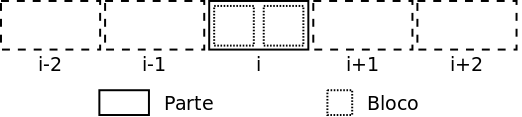
\includegraphics[width=0.64\textwidth]{partes.png}}
    \caption{trecho da seção de dados do torrent, com as divisões das partes e dos
    blocos}
    \label{fig:partes}
\end{figure}

Com esta mensagem, um \gls*{peer} pede por uma parte do \gls*{torrent}. A seção de dados
contém os seguintes números inteiros:

\begin{figure}[ht!]
    \centering
    \fbox{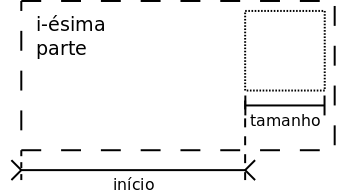
\includegraphics[width=0.64\textwidth]{request.png}}
    \caption{parâmetros da mensagem \emph{request} e seus significados}
    \label{fig:request}
\end{figure}

\begin{description}
    \item[índice:] índice da parte base $i$;
    \item[início:] deslocamento, em bytes, da posição do bloco da parte $i$ pedida; e
    \item[tamanho:] tamanho, em bytes, do bloco pedido.
\end{description}

\cfile[label="./libtransmission/peer-msgs.c:356"]{./Codes/chap3/037-request.c}

\subsubsection*{piece}

\textbf{piece:} \bverb|<tamanho=0009+X><ID da mensagem=7><dados=<índice><início><bloco>>|

Esta mensagem é a resposta para a requisição de um bloco por meio da mensagem
\emph{request}, tendo assinatura análoga, com exceção do trecho com os dados do bloco.
Assim, um \gls*{peer} envia um bloco de dados a outro.

\newpage
O tamanho da mensagem é variável, onde $X$ é o tamanho do segmento de dados, já que
este pode ter tamanhos diferentes entre mensagens diferentes. A seção de dados possui
os seguintes números inteiros:

\begin{description}
    \item[índice:] índice da parte base $i$;
    \item[início:] deslocamento, em bytes, da posição do bloco da parte $i$ pedido; e
    \item[bloco:] conteúdo dos dados do bloco.
\end{description}

\cfile[label="./libtransmission/peer-msgs.c:1093"]{./Codes/chap3/034-piece.c}

\newpage
\subsubsection*{cancel}

\textbf{cancel:} \bverb|<tamanho=0013><ID da mensagem=8><dados=<índice><início><tamanho>>|

A mensagem \emph{cancel} serve para cancelar a mensagem \emph{request} de mesmos
parâmetros. É mais utilizada durante o algoritmo de fim de jogo (página
\pageref{subsubsec:endgame}).

\cfile[label="./libtransmission/peer-msgs.c:372"]{./Codes/chap3/035-cancel.c}

\subsubsection*{port}

\textbf{port:} \bverb|<tamanho=0003><ID da mensagem=9><dados=porta>|

Para casos em que o \gls*{peer} estiver usando a função de \gls*{dht}, esta mensagem
serve para avisar ao receptor qual a porta de comunicação \gls*{tcp} é usada pelo
remetente para receber mensagens de \gls*{dht}. Com isso, é adicionado à tabela de
roteamento do receptor.

\cfile[label="./libtransmission/peer-msgs.c:387"]{./Codes/chap3/036-port.c}


%!TEX root = ../../tcc.tex

\newpage
\subsection*{Algoritmos de seleção de partes}

Por se tratar de um protocolo de troca de dados em partes, uma escolha ruim sobre quais
destas se adquirir primeiro, faz com que seja grande a possibilidade de um \gls*{peer}
baixar alguma parte que seja sempre ofertada por outros \glspl*{peer}
\cite{artigo:bittorrent}. Isso acarretará em não se ter nenhuma das partes que se
deseja. Assim, durante a troca das partes, um \gls*{peer} adota estratégias diferentes
para fornecer e receber blocos de dados, com o intuito de tentar otimizar a obtenção do
conjunto total de dados dos \glspl*{torrent}, e ajudar a difundir o conteúdo deste ao
resto do \gls*{swarm}.

As estratégias a seguir relacionadas são medidas que um \gls*{peer} BitTorrent pode
adotar, gerando efeitos em si mesmo, mas sem afetar outros \glspl*{peer}.

\subsubsection*{Random First Piece}

No início do download de um \gls*{torrent}, um \gls*{peer} não possui partes. Para que
comece a receber partes, ele avisa que é recém-chegado, e então algum membro do
\gls*{swarm} envia-no uma parte comum aleatoriamente (\emph{Random First Piece}). Dessa
forma, ele possuirá uma ``moeda de troca'', podendo com isso ajudar outros \glspl*{peer},
e assim, conseguir melhores condições de ser atendido. É importante que a parte seja
comum, pois dessa maneira será possível conseguir blocos de locais diferentes; se fosse
rara, seria mais difícil conseguir completá-la.

Após completar a primeira parte, o algoritmo passa para a estratégia de \emph{Rarest
First}.

\subsubsection*{Rarest First}
\label{subsubsec:rarest-first}

Nesta fase, o \gls*{peer} passa a pedir as partes mais raras primeiro
(\emph{Rarest First}). Para isso, utiliza os bitfields recebidos dos outros
\glspl*{peer}, mantendo-os atualizados a cada mensagem \bverb|have| que recebe. Feito
isso, das partes que são menos frequentes nos bifields, escolhe uma aleatoriamente,
devido ao fato de que uma parte rara poderia ser muito requisitada, o que seria
improdutivo. Da mesma forma, a estratégia de deixar partes mais comuns para serem
baixadas mais tarde não é prejudicial, pois a probabilidade de que um \gls*{peer}
deixará de ser interessante, por estar disponibilizando essas partes em um dado
momento, é reduzida.

É fácil ver que, enquanto um \gls*{seeder} não enviar todas as partes do \gls*{torrent}
que está fornecendo, não haverá nenhum \gls*{peer} que possa ter terminado de baixá-lo.
Assim, quando o \gls*{seeder} possuir capacidade de upload menor do que de seus
\glspl*{leecher}, será melhor que cada \gls*{leecher} baixe partes diferentes dos
outros, que maximizará o espalhamento dos dados e aliviará a carga sobre o \gls*{seeder},
justificando a prioridade em se fazer download das partes raras.

Em uma outra situação, o \gls*{seeder} pode sair da rede, tornando os \glspl*{leecher}
responsáveis pela distribuição do \gls*{torrent}. Com isso, corre-se o risco de alguma
parte se tornar indisponível. O \emph{rarest first} também ajuda neste caso, pois
replica as partes raras o mais rápido possível, reduzindo o risco do \gls*{torrent} se
tornar incompleto.

\subsubsection*{Strict Priority}

Cada parte é composta de blocos, que são os pacotes de dados trocados entre
\glspl*{peer}. Esta política de prioridade (\emph{Strict Priority}) faz com que, se um
bloco for requisitado, o restante dos blocos da mesma parte serão pedidos antes dos
blocos de outras partes, a fim de se ter partes completas o mais rápido possível.

\subsubsection*{Endgame Mode}
\label{subsubsec:endgame}

Próximo ao fim do download de um \gls*{torrent} (\emph{Endgame Mode}), a tendência é
que os últimos blocos de dados demorem, chegando aos poucos. Para agilizar isso, o
cliente entra no modo de fim de jogo, onde pede todos os blocos faltantes para todos os
\glspl*{peer}, enviando uma mensagem \bverb|cancel|, assim que o bloco for recebido,
para todos aqueles que não tiverem respondido à requisição, de modo a evitar despedício
de banda de rede na recepção redundante de dados.

\subsubsection*{Implementação do Transmission}

O Transmission implementa as partes desejadas e os blocos do \gls*{torrent} a serem
baixados como vetores. O vetor de partes é ordenado, utilizando seus campos auxiliares,
de forma que a parte mais importante que se deseja receber será requisitada antes. Ele
é usado para decidir quais blocos serão requisitados.

\cfile[label="./libtransmission/peer-mgr.c:172"]{./Codes/chap3/038-struct-weighted-piece.c}

Conforme são recebidas mensagens \bverb|have| e \bverb|bitfield| de outros \glspl*{peer},
ocorre o processamento da carga de dados dessas mensagens e a atualização das
informações das partes de cada remetente. Assim, o Transmission estima quais partes do
\gls*{torrent} são mais raras que outras, guardando essa informação no vetor de
replicações.

\cfile[label="./libtransmission/peer-mgr.c:1699"]{./Codes/chap3/041-peer-callback.c}

Essa informação é utilizada na reordenação desse vetor, utilizando a função da linguagem
C \sverb|qsort()|, que recebe em um dos parâmetros uma função comparadora. A função do
Transmission considera, nesta ordem:

\begin{enumerate}
    \item \emph{strict policy}: completude de uma parte;
    \item prioridade (assinalada manualmente pelo usuário): prioridade do usuário;
    \item \emph{rarest first}: raridade da parte; e
    \item \emph{random first piece}: aleatoriedade.
\end{enumerate}

\cfile[label="./libtransmission/peer-mgr.c:948"]{./Codes/chap3/044-compare-piece-weight.c}

Já o vetor de blocos mantém a lista dos blocos pedidos no momento da requisição e para
quem esta foi feita. Essa lista é usada para cancelar requisições que ficaram pendentes
por muito tempo ou para evitar requisições duplicadas antes do modo de fim de jogo.

\cfile[label="./libtransmission/peer-mgr.c:165"]{./Codes/chap3/039-struct-block-request.c}

Ambos os vetores são armazenados em uma estrutura que guarda essas e outras informações
sobre o \gls*{swarm} do \gls*{torrent} que está sendo baixado.

\cfile[label="./libtransmission/peer-mgr.c:187"]{./Codes/chap3/040-struct-swarm.c}

Eventualmente, o Transmission verifica a necessidade e a capacidade de enviar pedidos
de blocos. Caso seja possível, realiza o processamento da lista de partes, montando uma
lista de blocos a serem requisitados.

\newpage
\cfile[label="./libtransmission/peer-mgr.c:1324"]{./Codes/chap3/042-peer-mgr-getreqs.c}

\newpage
Tendo criado a lista de blocos, os requisita.

\cfile[label="./libtransmission/peer-msgs.c:1874"]{./Codes/chap3/043-update-block-reqs.c}

Durante a execução da função de criação da lista de blocos a serem pedidos, existe a
verificação da completude do \gls*{torrent}, onde se percebe que a quantidade de bytes
requisitados já é maior do que a quantidade de bytes que faltam ser baixados. Eis que o
modo de fim de jogo se inicia, quando é calculada a capacidade de um novo \gls*{peer}
receber e atender a nova requisição de bloco, de forma melhor ou igual à taxa que
atuais \glspl*{peer} estão fazendo.

\cfile[label="./libtransmission/peer-mgr.c:878"]{./Codes/chap3/045-test-end-game.c}
\cfile[label="./libtransmission/peer-mgr.c:887"]{./Codes/chap3/046-update-end-game.c}

%!TEX root = ../../tcc.tex

\newpage
\subsection*{Algoritmos de enforcamento}

Além das estratégias mostradas, existem outras que são as formas com que um \gls*{peer}
se relacionará com seus vizinhos. Cada \gls*{peer} é responsável por melhorar suas
taxas de download e, para isso, baixam partes de quem eles conseguem e escolhem para
quais enviará outras partes, de modo a mostrar cooperação. Caso a escolha seja de não
cooperar, um \gls*{peer} ``enforca'' (\emph{choke}) outro, o que implica num
cancelamento temporário do envio de partes do primeiro para o segundo. O recebimento de
partes continuará normalmente e a conexão não precisará ser rediscutida quando o
enforcamento terminar.

O enforcamento (ou \emph{choking}) não faz parte do protocolo de mensagens, mas é
necessário para a boa performance do protocolo. Um bom algoritmo de \emph{choking}, que
se utilize de todos os recursos disponíveis, traz boas condições para todos os
\glspl*{peer} cooperativos e é resistente contra aqueles que só fazem download.

\subsubsection*{Eficiência de Pareto}

Sistemas \emph{pareto eficientes} \cite{wiki:pareto} são aqueles onde duas entidades
não podem fazer trocas e ficar mais ``felizes'' que antes. Em termos de Ciência da
Computação, buscar a eficiência de Pareto é usar um algoritmo de otimização local onde
as entidades procurem meios de melhorar mutuamente, que convergirão a uma situação ótima
global. No contexto do BitTorrent, se dois \glspl*{peer} não estão tendo vantagem
recíproca por enviar partes, eles podem começar a trocar partes entre si, de modo a
conseguir taxas de download melhores do que as anteriores.

\subsubsection*{Algoritmo de choking}

Cada \gls*{peer} fará \emph{unchoke} de quatro \glspl*{peer} (geralmente), ou seja,
sempre deixará livres de enforcamento cerca de quatro \glspl*{peer}. Com isso, o
problema passará a ser escolher quais deles fazer, deixando que o \gls*{tcp} controle o
congestionamento de banda. Essa escolha é baseada estritamente na taxa de download,
calculando-se a média dessa taxa durante vinte segundos. Antigamente, esse cálculo era
feito sobre quantidades transferidas a longos prazos, mas notou-se que era uma medida
fraca por causa das variações de largura da banda de rede.

Para evitar que recursos sejam desperdiçados pelo rápido \emph{choke} e \emph{unchoke}
de \glspl*{peer}, um cálculo é realizado a cada dez segundos a fim de saber quem
sofrerá o \emph{choke}, deixando a situação atual como está até o próximo intervalo
acabar. Esse tempo é suficiente para que o \gls*{tcp} acelere transferências até sua
capacidade total.

\subsubsection*{Optimistic Unchoking}

Fazer upload para \glspl*{peer} que possuem as melhores taxas de download não é tarefa
fácil, pois não há meios de se descobrir conexões melhores. Para tentar contornar esse
problema, um \gls*{peer} será escolhido para ser alvo de um ``\emph{unchoke} otimista''
(\emph{Optimistic Unchoking}), que é um \emph{unchoke} independentemente da taxa de
download que ele provê.

A escolha do \gls*{peer} ocorrerá a cada trinta segundos (após o terceiro ciclo de
\emph{choke}). Esse tempo é suficiente para que o \gls*{peer} escolhido tome a
iniciativa de colaborar enviando partes, sendo recompensado com novas, e essas
transmissões alcancem altas taxas de upload e download.

Este algoritmo objetiva, portanto, incentivar a cooperação entre \glspl*{peer}.

\subsubsection*{Anti-snubbing}

Eventualmente, um \gls*{peer} sofrerá \emph{choke} de todos os \glspl*{peer} de onde
estava fazendo download. Nesses casos, terá taxas de download ruins até que um
\emph{unchoke} otimista seja executado.

Quando ficar mais de um minuto sem receber nenhuma parte de um outro \gls*{peer}, o
\gls*{peer} que não recebeu nada perceberá que foi censurado (\emph{snubbed}), e
retaliará deixando de enviar partes para quem o censurou \emph{Anti-snubbing}, a menos
que ele seja sorteado em um \emph{unchoke} otimista. Dessa forma, vários unchokes
otimistas serão executados simultaneamente, o que implicará na recuperação das taxas de
download.

\subsubsection*{Upload Only}

Enquanto um \gls*{peer} ainda não recebeu todas as partes do \gls*{torrent}, ele
priorizará para quem enviará as que ele possui, de acordo com as taxas de download que
ele atinge com os outros \glspl*{peer}. Isso acelerará a disseminação do \gls*{torrent}.
Porém, quando tiver recebido todas as partes, o \gls*{peer} manterá a rápida
disseminação do \gls*{torrent}, priorizando os \glspl*{peer} que alcançam altas taxas de
download com ele, maximizando sua taxa de upload.

\subsubsection*{Implementação do Transmission}

Quando um \gls*{torrent} é executado, e em intervalos de dez segundos, o Transmission
executa uma função que faz os \emph{chokes} de upload e também verifica os downloads.

\cfile[label="./libtransmission/peer-mgr.c:3167"]{./Codes/chap3/047-rechoke-pulse.c}

Primeiro, verifica os uploads: a cada execução da função, verificará se será um turno de
\emph{unchoke} otimista, que durará quatro execuções. Além disso, o vetor de
\glspl*{peer} será analisado para se obter informações, guardadas em um vetor
temporário, que ajudarão na decisão de quais desses \glspl*{peer} passarão a ser
\emph{choked}.

\cfile[label="./libtransmission/peer-mgr.c:3057"]{./Codes/chap3/048-rechoke-up1.c}

A ordenação é feita com \sverb|qsort()| usando uma função comparadora que classifica os
\glspl*{peer} considerando, nesta ordem:

\begin{enumerate}
    \item velocidade de transferência de dados (download e upload);
    \item estado de \emph{choke}: preferência por \emph{unchoked}; e
    \item aleatoriedade.
\end{enumerate}

\cfile[label="./libtransmission/peer-mgr.c:2993"]{./Codes/chap3/049-compare-choke.c}

Então, trata o vetor temporário: os melhores \glspl*{peer} mudarão seu estado para
\emph{unchoked}, enquanto o restante permanecerá \emph{choked}. Além disso, no caso de
um rodada de \emph{unchoke} otimista, sorteará um dos \glspl*{peer} para ter a sua vez.

\cfile[label="./libtransmission/peer-mgr.c:3057"]{./Codes/chap3/050-rechoke-up2.c}

Depois, trata os downloads: primeiro, calculará para quantos \glspl*{peer} mandará
mensagens \bverb|interested|, usando como base as estatísticas de pedidos de blocos e
quais deles foram cancelados, dentro de limites de bom funcionamento.

\cfile[label="./libtransmission/peer-mgr.c:2833"]{./Codes/chap3/051-rechoke-down1.c}

Após saber o limite de \glspl*{peer}, o Transmission procurará quais deles contatará, de
acordo com as partes que lhe faltam. Para isso, montará um vetor com informações dos
\glspl*{peer}, ordenando-o pela função \sverb|qsort()|, e fornecerá uma função
comparadora que avaliará os critérios:

\begin{enumerate}
    \item estado de \emph{choke}: se um \gls*{peer} tiver cancelado 10\% (ou menos) dos
        pedidos de blocos, terá preferência sobre os outros; e
    \item aleatoriedade.
\end{enumerate}

\cfile[label="./libtransmission/peer-mgr.c:2813"]{./Codes/chap3/053-enum-rechoke.c}

\cfile[label="./libtransmission/peer-mgr.c:2820"]{./Codes/chap3/052-compare-rechoke.c}

\cfile[label="./libtransmission/peer-mgr.c:2833"]{./Codes/chap3/054-rechoke-down2.c}